\documentclass[aspectratio=1610]{beamer}

\usepackage[utf8]{inputenc}
\usepackage[russian]{babel}
\usepackage[OT1]{fontenc}
\usepackage{amsmath}
\usepackage{amsfonts}
\usepackage{amssymb}
\usepackage{makeidx}
\usepackage{graphicx}
\usepackage{xcolor}
\usepackage{multirow}
\usepackage{framed}
\definecolor{shadecolor}{cmyk}{0,0,0,1}
\usepackage{hyperref}
\usepackage[normalem]{ulem}
\usepackage{listings}

\usefonttheme{structurebold}

\definecolor{mailblue}{RGB}{1, 75, 135}
\definecolor{mailorange}{RGB}{247, 163, 27}
\setbeamercolor{normal text}{bg=mailblue,fg=white}
\setbeamercolor{title}{fg=mailorange}
\setbeamercolor{frametitle}{fg=mailorange}
\setbeamercolor{titlelike}{fg=mailorange}
\setbeamercolor{item}{fg=mailorange}
\setbeamercolor{eecks} {bg=white, fg=mailblue}

\setbeamercolor{block title}{bg=white,fg=mailblue,shadow=false}
\setbeamercolor{block body}{bg=white,fg=mailblue,shadow=false}

\setbeamertemplate{itemize/enumerate body begin}{\normalsize}
\setbeamertemplate{itemize/enumerate subbody begin}{\normalsize}
\setbeamertemplate{itemize/enumerate subsubbody begin}{\normalsize}

\setlength{\parskip}{1em}

\titlegraphic{
   
\includegraphics[width=3cm]{images/logo-mail-ru.png}
}

\author{Nikolay Anokhin}
\title{MapReduce programming model for Big Data analysis}
\date{}

\beamertemplatenavigationsymbolsempty

\begin{document}

\maketitle

% #####################
\section{Problem statement}
% #####################

\begin{frame}{Advertisement on the Web}

\begin{center}
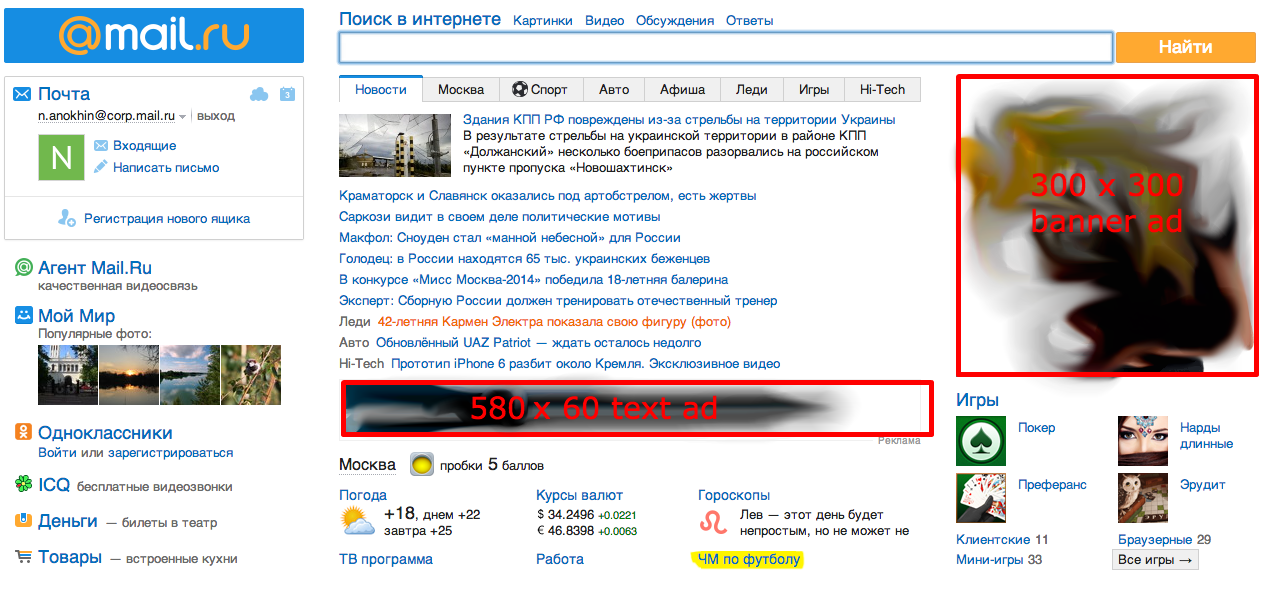
\includegraphics[scale=0.3]{images/banners.png}
\end{center}
%Introduce the concept of web-advertising. Point out that it requires optimisation based on a user's interests

\end{frame}

\begin{frame}{It's all about users (and money)\footnote{Image source: \href{http://www.deviantart.com/art/Geek-Usopp-119715834}{Deviantart}}}

\begin{center}
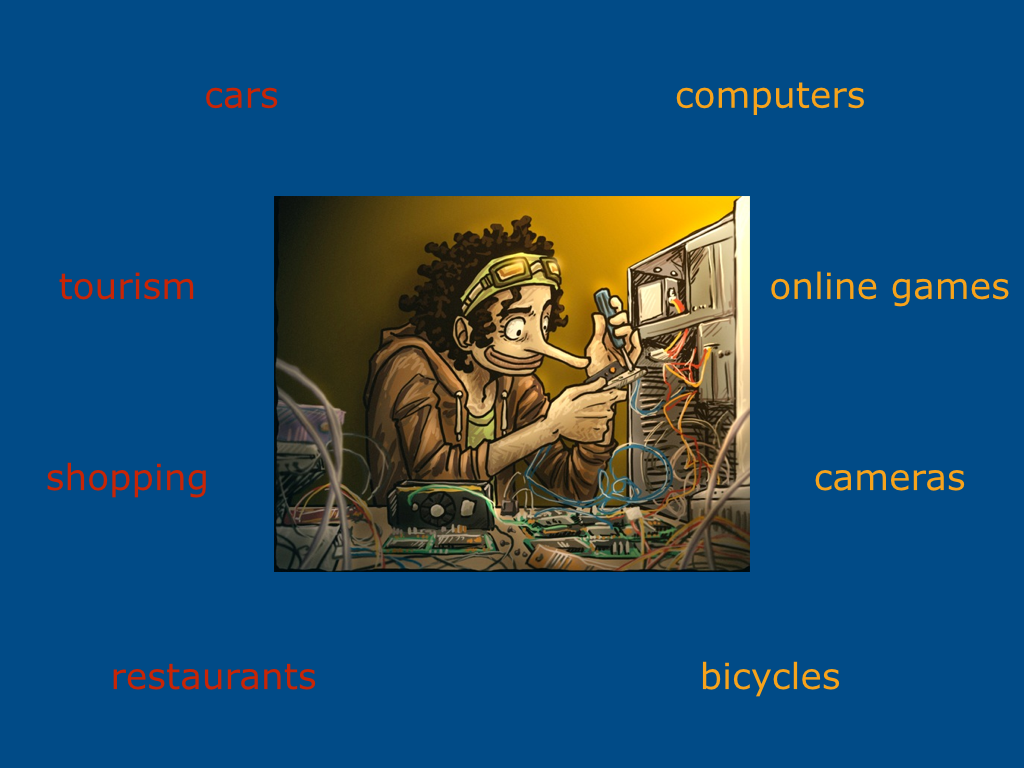
\includegraphics[scale=0.3]{images/geek.png}
\end{center}

%Give an example of a user profile, for e.g. a geek, and explain how this profile can be used in online  advertising

%Can we infer the profile from our data?

\end{frame}

\begin{frame}{The Data: user access logs}

\begin{center}
\begin{tabular}{c c l c}
\bf User ID & \bf Timestamp & \bf URL & \bf Etc. \\
\hline
A1B2C3D4 & 2014-07-01 13:11:37 & http://auto.mail.ru/toyota & M/27/... \\
A1B2C3D4 & 2014-07-01 13:20:45 & http://example.com?id=football & M/27/... \\
A1B2C3D4 & 2014-07-02 00:25:10 & http://somesite.com/index.php & M/27/... \\
\ldots & & & \\
F9E8D7C6 & 2014-06-30 18:01:12 & http://my-little-pony.com/ & F/19/... \\
F9E8D7C6 & 2014-06-30 18:10:51 & http://afisha.mail.ry/twilight & F/19/... \\
\end{tabular}

{\bf Text log files -- about 300 G/day (and growing)}
\end{center}

\end{frame}

\begin{frame}{Some immediate conclusions}

\begin{center}
\begin{tabular}{c c l c}
\bf User ID & \bf Timestamp & \bf URL & \bf Etc. \\
\hline
A1B2C3D4 & 2014-07-01 13:11:37 & http://{\color{mailorange}auto}.mail.ru/{\color{mailorange}toyota} & M/27/... \\
A1B2C3D4 & 2014-07-01 13:20:45 & http://example.com?id={\color{mailorange}football} & M/27/... \\
A1B2C3D4 & 2014-07-02 00:25:10 & http://{\color{mailorange}somesite}.com/index.php & M/27/... \\
\end{tabular}
\begin{huge}
\[
\downarrow
\]
\end{huge}
A1B2C3D4: \quad auto, toyota, football, somesite
\end{center}

%Problems: can't process automatically, too much data, interests are not well-defined

\end{frame}

% #####################
\section{LDA}
% #####################

\begin{frame}{Multinomial distribution}

Let $\theta = (\theta_1, \ldots, \theta_k)$ be the probability mass function (PMF) for a set of $k$ events, i.e.
\[
\forall i = 1, \ldots, k: \; \theta_i \geqslant 0 \quad \text{and} \quad \sum_{i=1}^k \theta_i = 1
\]
Binomial distribution ($k = 2, \; \theta_1 = q, \; \theta_2 = 1- q$)
\[
p(x | n , q) = \frac{n!}{x! (n-x)!} q^{x} (1 - q)^{n-x}
\]
Multinomial distribution
\[
p(x_1, \ldots, x_k | n, \theta_1, \ldots, \theta_k) = \frac{n!}{x_1! \ldots x_k!} \prod_{i=1}^k \theta_i^{x_i}
\]

\end{frame}

\begin{frame}{Dirichlet distribution}

Let
\begin{enumerate}
\item $\Theta = (\Theta_1, \ldots, \Theta_k)$ be a random PMF, i.e. $ \forall i: \; \Theta_i \geqslant 0 $ and $\sum_{i=1}^k \Theta_i = 1$
\item $\alpha = (\alpha_1, \ldots, \alpha_k)$ be a vector, s.t. $\forall i: \; \alpha_i > 0$ and $\alpha_0 = \sum_{i=1}^k \alpha_i$
\end{enumerate}

{Then $\Theta$ is said to have {\it Dirichlet distribution} with parameter $\alpha$, iff}
\[
p(\theta_1, \ldots, \theta_k | \alpha_1, \ldots, \alpha_k) = \begin{cases}
\frac{\Gamma(\alpha_0)}{\prod_{i=1}^k \Gamma(\alpha_i)} \prod_{i=1}^k \theta_i^{\alpha_i - 1} \qquad \text{if} \;\theta\; \text{-- PMF} \\
0  \;\qquad\qquad\qquad\qquad\qquad\text{otherwise}
\end{cases}
\]
where
\[
\forall s > 0: \Gamma(s + 1) = s \Gamma(s)
\]

\end{frame}

\begin{frame}{Dirichlet distribution}

\begin{center}
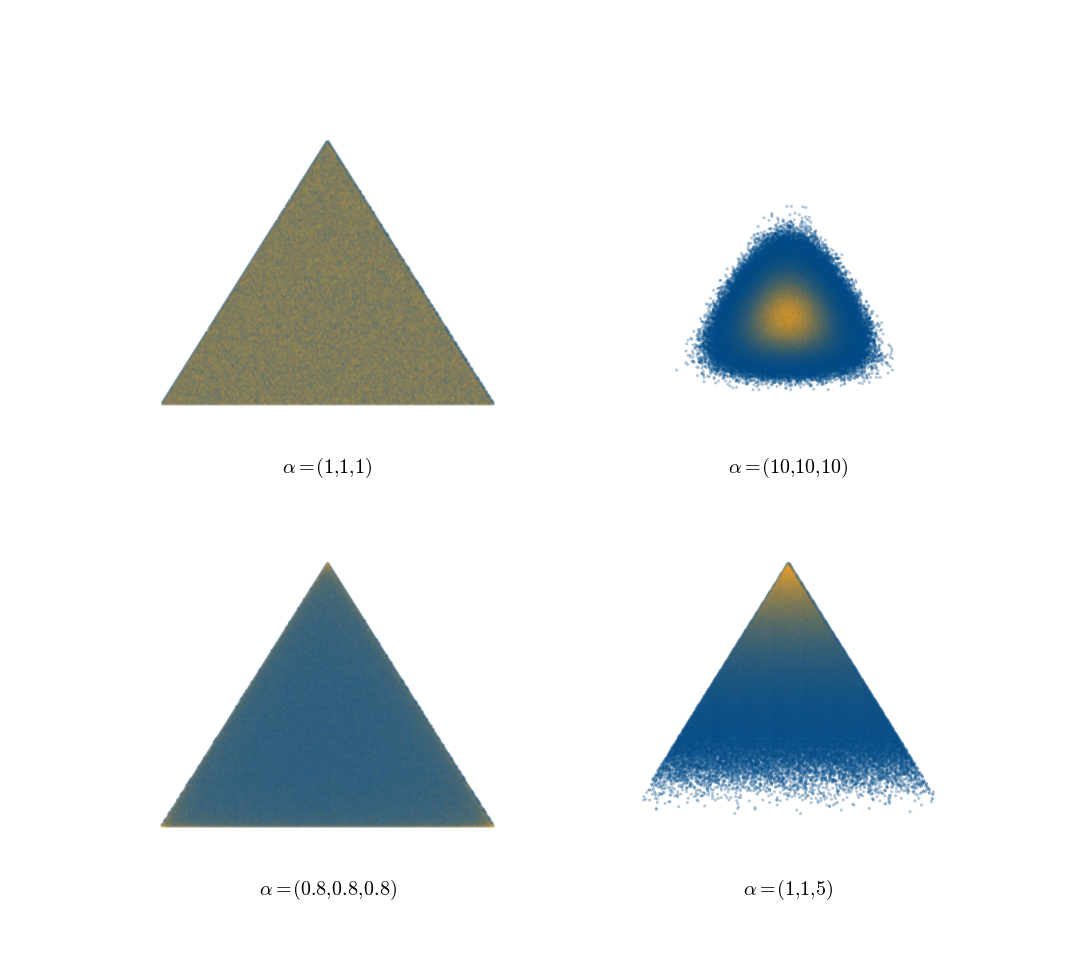
\includegraphics[scale=0.33]{images/dirichlet.png}
\end{center}

\end{frame}

\begin{frame}{Latent Dirichlet Allocation\footnote{Latent Dirichlet Allocation // Blei et. al.}}

\begin{itemize}
\item Let there be $M$ users, each user $u$ is represented by a bag of $N_u$ tokens
\item Let the number of {\it topics} (user interests) be given and equal to $K$
\end{itemize}

Generative model
\begin{enumerate}[I]
\item For each topic draw a topic distribution $\beta_k \sim \text{Dir}(\eta_k), \; k \in 1, \ldots K$
\item For each user $u \in 1, \ldots, M$:
\begin{enumerate}[1]
\item Draw the user's topic distribution $\theta_u \sim \text{Dir}(\alpha)$
\item For each potential token $t \in 1, \ldots, N_u$:
\begin{enumerate}[2.1]
\item Choose the token's topic assignment $z_{u, t} \sim \text{Multl}(\theta_u)$
\item Choose the token $w_{u, t} \sim \text{Mult}(\beta_{z_{u, t}})$
\end{enumerate}
\end{enumerate}
\end{enumerate}

\end{frame}

\begin{frame}{Generative model}

\begin{columns}[C]
    \begin{column}{.5\textwidth} 
    \begin{multline*}    
     p(\mathbf{w}, \theta,\beta, \mathbf{z} | \alpha, \eta) = \\
    = p(\theta | \alpha) \prod_{t=1}^N p(z_t | \theta) p(\beta | \eta) p(w_t | z_t, \beta)
    \end{multline*}
    
    \vspace{2em}
    \[
    p(\theta, \beta, \mathbf{z} | \mathbf{w}, \alpha, \eta) = \frac{p(\theta,\beta, \mathbf{z}, \mathbf{w} | \alpha, \eta)}{p(\mathbf{w} | \alpha, \eta)}
    \]
    \end{column}
    \begin{column}{.5\textwidth} 
    \vspace{0em}
    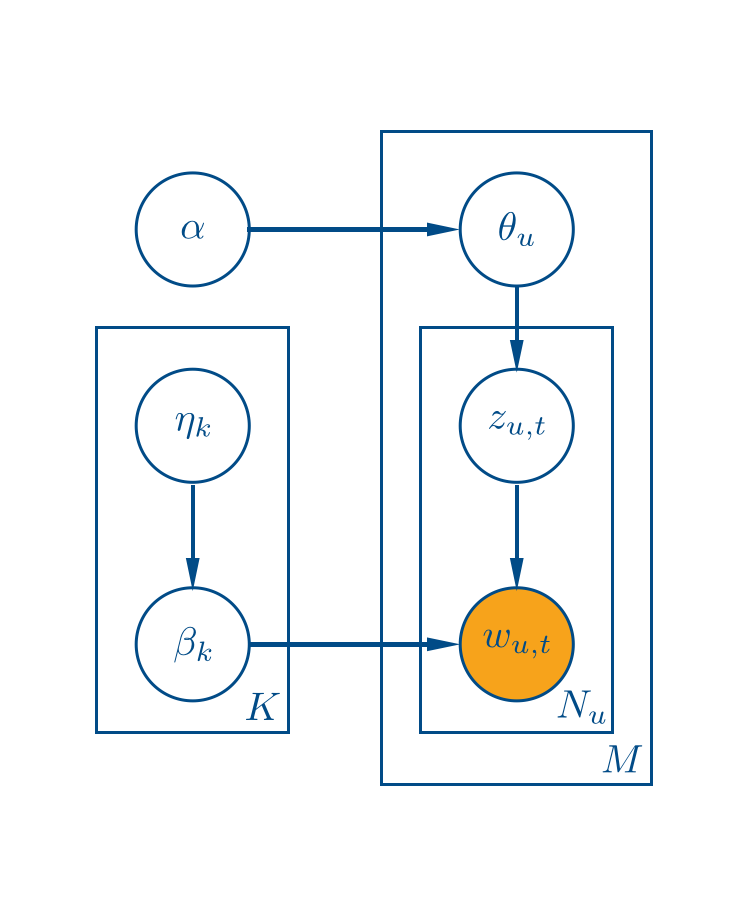
\includegraphics[scale=0.25]{images/gm.png}   
    \end{column}
\end{columns}

\end{frame}

\begin{frame}{Variational inference}

\begin{columns}[C]
    \begin{column}{.5\textwidth}
    \begin{multline*} 
    q(\theta, \beta, \mathbf{z}) = \prod_{k=1}^K \text{Dir}(\beta_k | \lambda_k) \times \\  \times \prod_{u=1}^M\text{Dir}(\theta_u | \gamma_u) \prod_{t=1}^N \text{Mult}(z_{u,t} | \varphi_{u,t})
    \end{multline*}
    
    \vspace{2em}
    Maximizing the ELBO...
    \[
    \mathcal{L} = E_q \left[\log(p(\mathbf{w}, \theta, \beta, \mathbf{z})\right] - E_q \left[\log q(\theta, \beta, \mathbf{z}) \right]
    \]    
    ...is the same as minimising KL-divergence
    \[
    KL(q || p) = E_q \left[ \log\frac{q(\theta, \beta, \mathbf{z})}{p(\theta, \beta, \mathbf{z} | \mathbf{w})}\right]
    \]
    \end{column}
    \begin{column}{.5\textwidth} 
    \vspace{0em}
    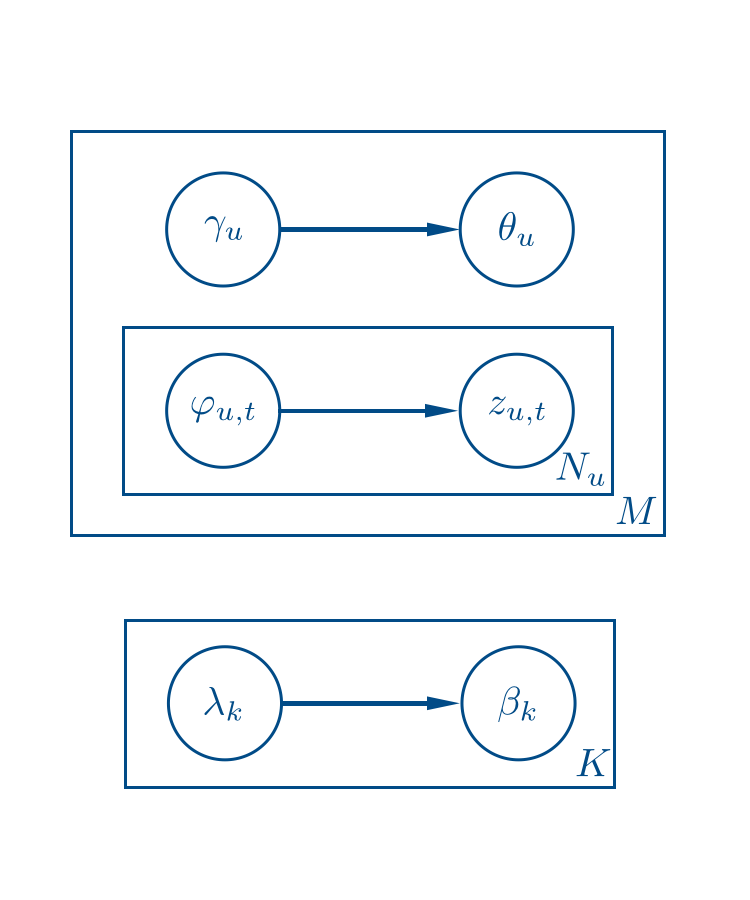
\includegraphics[scale=0.25]{images/vi.png}   
    \end{column}
\end{columns}

\end{frame}

\begin{frame}{Variational EM}

\begin{itemize}
\item[E1] For each user, given $\alpha$ and $\lambda$, update $\varphi$ and $\gamma$
\[
\varphi_{t,k} \propto E_q[\beta_{t,k}] \exp \left( \Psi(\gamma_l) \right)
\]
\[
\gamma_k = \alpha_k + \sum_{w=1}^N \varphi_{t,k}
\]
\item[E2] Update $\lambda$ for each topic, using the obtained $\varphi$ 
\[
\lambda_{t,k} =\eta_{t,k} + \sum_{u=1}^M w_{t}^{(u)} \varphi_{t,k}^{(u)}
\]
\item[M] Maximise lower bound of the data log likelihood w.r.t. to $\alpha$ using Newton-Raphson method
\end{itemize}

% #####################
\section{MapReduce on Hadoop}
% #####################

\end{frame}

\begin{frame}{Storing the data --- HDFS\footnote{Image source: \href{http://hadoop.apache.org/docs/r1.2.1/hdfs_design.html}{HDFS architecture guide}}}

\begin{center}
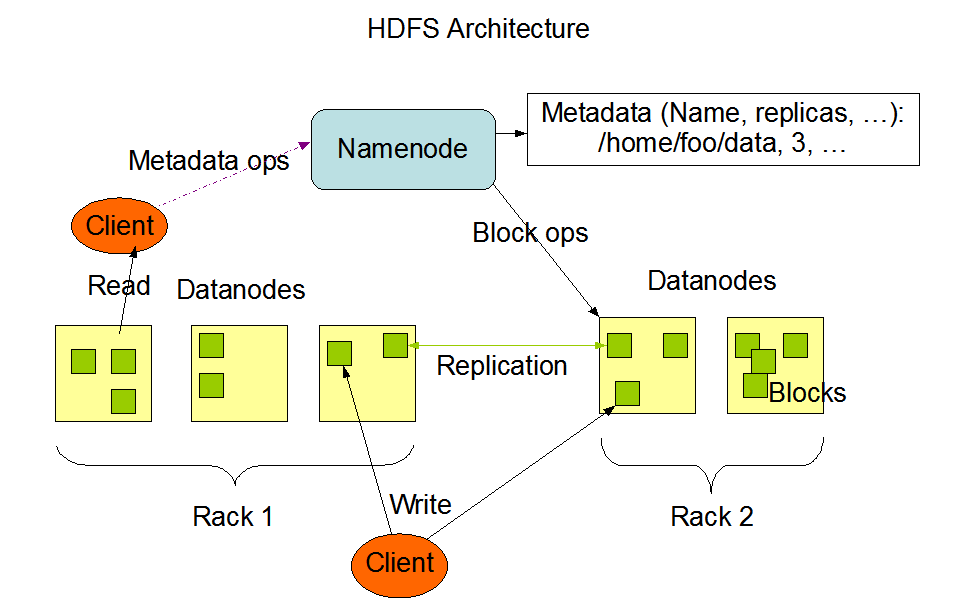
\includegraphics[scale=0.33]{images/hdfs.png}
\end{center}

\end{frame}

\begin{frame}[fragile]{Processing the data --- Hadoop MapReduce\footnote{MapReduce: Simplified Data Processing on Large Clusters // Jeffrey Dean, Sanjay Ghemawat}}

\begin{center}
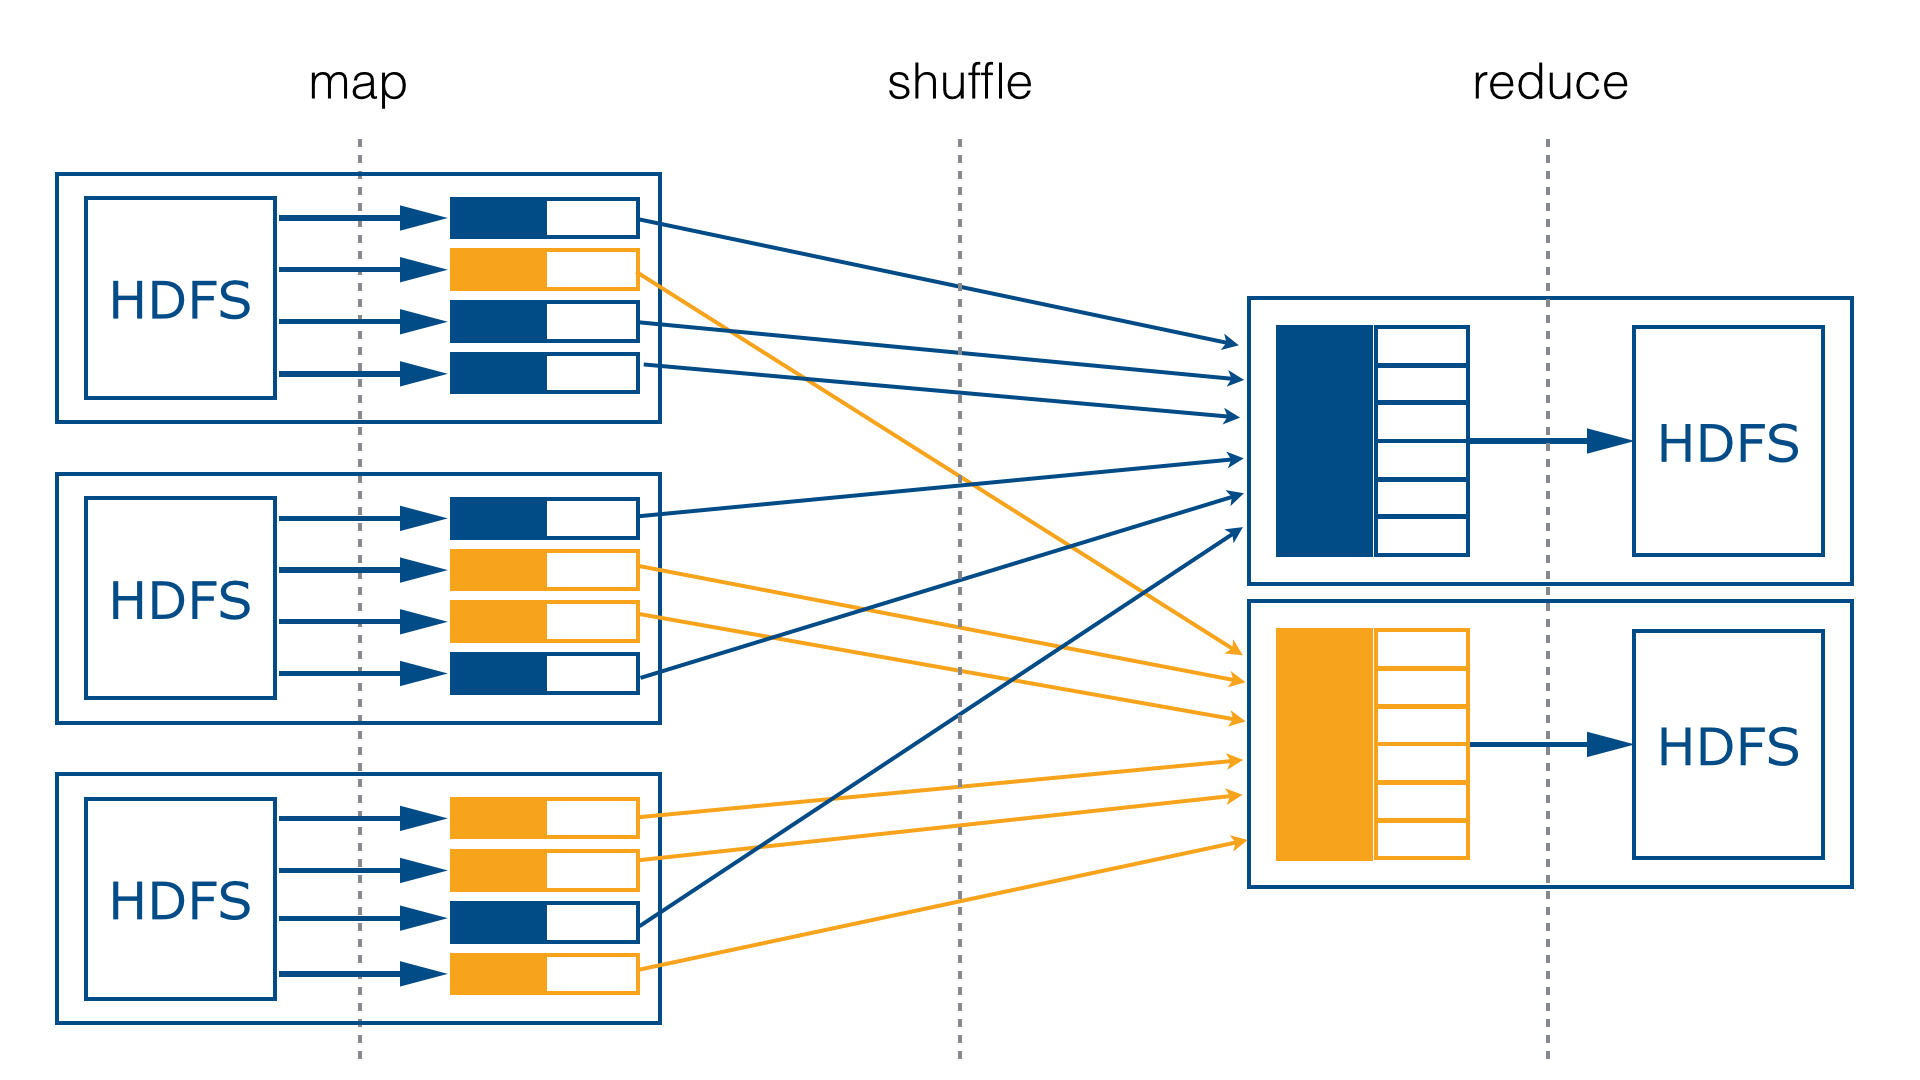
\includegraphics[scale=0.16]{images/mr.png}
\end{center}
\begin{verbatim}
map( Key1, Value1 ):  List[( Key2, Value2 )]
reduce( Key2, List[Value2] ):  List[( Key3, Value3 )]

\end{verbatim}

\end{frame}

\begin{frame}[fragile]{LDA -- map\footnote{Mr. LDA: A Flexible Large Scale Topic Modeling Package
using Variational Inference in MapReduce // Zhai et. al.}}

\begin{columns}[C]
    \begin{column}{.5\textwidth}    
\begin{small}

{\bf Input:} \\
KEY -- user ID $u \in [1, M]$ \\
VALUE -- user tokens \\
{\bf Configure} \\
1: Load in $\alpha$, $\lambda$ and $\gamma$ from distributed cache  \\
2: Normalize $\lambda$ for every topic \\
{\bf Map} \\
1: Initialize a zero $V \times K$-dimensional matrix $\varphi$ \\
2: Initialize a zero $K$-dimensional row vector $\sigma$ \\
3: Read in user logs $\| t_1, t_2, . . . , w_N \|$ \\
4: repeat \\
5: \;\;for all $t \in [1, N]$ do \\
6: \;\;\;\;for all $k \in [1, K]$ do \\
7: \;\;\;\;\;\;Update $\varphi_{t,k} = \frac{\lambda_{t,k}}{\sum_t \lambda_{t,k}} \exp \left( \Psi(\gamma_k) \right)$ \\
8: \;\;\;\;end for \\
9: \;\;\;\;Normalize $\varphi_t$, set $\sigma = \sigma + w_t \varphi_{t,*}$ \\
10: \;end for \\
11: \;Update row vector $\gamma_{u,*} = \alpha + \sigma$ \\
12: until convergence 

\end{small}    
    \end{column}
    \begin{column}{.4\textwidth} 
\begin{small}

13: for all $k \in [1, K]$ do \\
14: \;\;for all $t \in [1, N]$ do \\
15: \;\;\;\;Emit $<k, t>$ : $w_t \varphi_{t,k}$ \\
16: \;\;end for \\
17: Emit $<k, u>$ : $\gamma_{u,k}$ to file \\
18: end for 

\end{small}
    \end{column}
\end{columns}

\end{frame}

\begin{frame}[fragile]{LDA -- reduce}

\begin{small}

{\bf Input:} \\
KEY - key pair $<p_{left}, p_{right} >$ \\
VALUE - an iterator $\mathcal{I}$ over sequence of values \\
{\bf Reduce} \\
1: Compute the sum $\sigma$ over all values in the sequence $\mathcal{I}$ ($\sigma$ is
unnormalized $\lambda$) \\
2: Emit  $<p_{left}, p_{right} >$ : $\sigma$

\end{small}

\end{frame}

\begin{frame}{Running LDA}


\begin{columns}[C]
    \begin{column}{.5\textwidth} 
    \vspace{2em}
  \begin{tabular}{ |l|l| }
  \hline
  \multicolumn{2}{|c|}{\bf Typical machine config} \\  
  \hline \hline
  processors & 2 x Intel(R) Xeon(R) 2.00GHz \\
  cores & 12 \\
  threads & 24 \\
  RAM & 32 GB \\
  HDD & 4-8 TB \\
  \hline \hline
  \multicolumn{2}{|c|}{\bf 30 machines in cluster} \\
  \hline
  \end{tabular}
    \end{column}
    \begin{column}{.5\textwidth} 
    Typical data: 10-days user logs \\
    Typical run time: 6 hours \\
    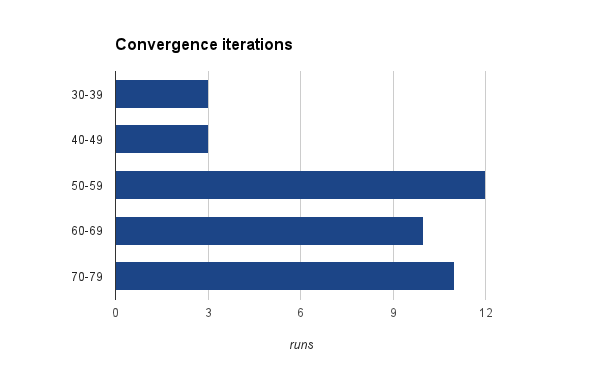
\includegraphics[scale=0.33]{images/iterations.png}   
    \end{column}    
\end{columns}

\end{frame}

\begin{frame}{Modelling results}

\begin{center}
\begin{tabular}{c c c c c c c c}
topic1 & topic2 & topic3 & topic4 & topic5 & topic6 \\
\hline
book & klass & mobile & avito & krasnoyarsk & china \\
books & reshebnik & svyaznoy & kvartiry & tyumen & meta \\
loveread & class & phone & doma & tomsk & shared \\
knigi & megabotan & telefony & prodam & kemerovo & links \\
read & resh & nokia & dachi & surgut & maincat \\
author & slovo & phones & kottedzhi & barnaul & linkwall \\
litmir & algebra & iphone & nedvizhimost & nizhnevartovsk & nakanune \\
labirint & yazyk & samsung & sdam & krsk & razvezlo \\
authors & reshebniki & catalog & oblast & novokuznetsk & poster \\
tululu & otbet & allnokia & komnaty & kurgan & readme
\end{tabular}
\end{center}

\end{frame}

\begin{frame}{Conclusions and Future Work}

\begin{itemize}
\item LDA is an appropriate model for Internet user's interests
\item Variational EM is an efficient algorithm for LDA parameter estimation
\item Variational EM is easy to parallelise using MapReduce paradigm
\end{itemize}

\vspace{1em}
\begin{itemize}
\item Profile prediction for a new user
\item Topics as features in data mining tasks
\end{itemize}

\end{frame}

\begin{frame}

\begin{center}
{\Huge\color{mailorange}Q\&A} \\
Nikolay Anokhin \\
\href{mailto:n.anokhin@corp.mail.ru}{n.anokhin@corp.mail.ru}
\end{center}

\end{frame}

\end{document}